% !TEX TS-program = xelatex
% !TEX encoding = UTF-8 Unicode

\documentclass[a4paper,10pt]{article}

\usepackage[english]{babel}
\usepackage{graphicx}
\usepackage{subcaption}
\usepackage{wrapfig}
\usepackage{amsmath}
\usepackage[hidelinks]{hyperref}
\hypersetup{
  unicode=true,
  pdftitle={Robotics paper},
  pdfsubject={Drowbot - A Suspended Polar Plotting Robot},
  pdfauthor={Micky Faas, Koen Putman},
  colorlinks=false,
  breaklinks=true
}
\usepackage{fontspec}
\defaultfontfeatures{Ligatures=TeX}
\usepackage[small,sf,bf]{titlesec}
% Times New Roman takes up less space so we can fit more text in fewer pages :)
\setromanfont{Times New Roman}
\setsansfont{Arial}
\setmonofont[Color={0019D4}]{Courier New}


% TODO: Add more citations in general because the paper is too long anyway
% TODO: clean the code a bit to make sure it's deliverable

\title{\vspace{-7em}

\includegraphics[scale=.85]{img/logo.png} \\ \vspace{.5em}
%\huge Drowbot 
\Large \sffamily{A Suspended Polar Plotting Robot}}

% TODO: Whoops I don't know your student number
% No problem, I don't know it either :)
\author{Micky Faas (s1407937) \and Koen Putman (s1305557)}
\date{}

\begin{document}
\maketitle
\begin{abstract}
%TODO: Actually write this
% Micky: zo ouwehoer ik mijzelf dus een weg door het leven...
In the past, plotting-devices were usually very expensive and specialistic equipment used by big printing studios. In recent years, the emergence of affordable embedded platforms such as Arduino as RaspberryPi have given rise to a myriad of plotters that are available to the general public and DIY-community. Those plotters are used by hobbyists, tinkerers, print-makers and also artists wanting to explore the boundaries of man-machine synergy. What most of these plotters have in common is that they are unidirectional devices: they simply execute drawing instructions sent by their operator and perform them. We introduce Drowbot, a bidirectional polar plotter. By using optical feedback, Drowbot can expand, adapt and interpolate directly on the canvas - allowing Drowbot to become a co-author rather than a tool.

%%% Original abstract from long ago
% There exist many different drawing- and writing robots. Examples
% include Axibot [1] or [2]. The most common constructions are either arm-based
% (single arm holding a pen) or have a plotter/CNC-style three-axis position pen.
% Practical implementation often utilize the GCode protocol to send drawing
% instructions to the robot; the robot itself lacks any ‘intelligence’, which basically
% makes it a printer/plotting-device. The ‘Maestrobot’ differentiates itself by being
% able to create its output untethered. It is equipped not only with a pen/marking-
% tool, but also with a simple optical sensor (infrared-led-photodiode). Using
% this sensor, the Maestrobot can ‘see’ what is already on the paper and use this
% information to decide where/what to draw next. Different algorithms could
% be suitable to add ‘intelligence’ to the robot’s drawing expertise. For example,
% cellular automata could be used to finish a given start sequence or the input could
% be combined with Perlin noise to create interesting textures. Eventually the
% robot could be used to perform certain difficult or tedious tasks in human-made
% art. These include repeating structures, fractals or extremely fine lines, given an
% algorithm specified by the artist.
% [1] https://www.axidraw.com/
% [2] https://www.thingiverse.com/thing:2349232
\end{abstract}

\section{Introduction}
\label{sec:intro}

% Micky: ik knip dit er even uit, we hebben *veel* teveel pagina's en dit staat ook soort-van in de abstract
%While some might consider drawing a distinctly human art form,
%many tools have been devised to assist in the process.
%In recent years there has been a shift to digital with drawing
%tablets and drawing software and it is not unusual for a drawing
%to never exist outside of the digital realm.
%This digital realm is very convenient, but why stop there.
%Our increasingly digital lives have brought us electronics that
%allow the digital to act in the real world, including the robot.

Many drawing robots have been devised to automate tedious and
repetitive parts of the artistic (printing-) process.
These include drawings arms and three-axis CNC-like solutions that
act as some form of plotter.
But we believe that robots do not have to be deterministic plotters
and wanted to see if they could interact with artwork and produce
drawings without pre-programmed or direct control.
Is it viable to give a drawing robot some agency to produce some
form of art on its own?

\section{Project Overview}
\label{sec:overview}
% Description and goals of the project

We set out to create a drawing robot that is partially controlled by
optical feedback.
With our limited amount of time and a live prototype presentation
on the horizon we had to set some constraints to make this possible.

Given that the live demo was held in a classroom the only viable drawing
surface was the blackboard, as transporting a large amount of surface
to draw on was infeasible.

Using the vertically mounted blackboard as surface and chalk as
end-effector seemed to have left us with a single viable approach: 
using a suspended drawing platform or \emph{gondola} attached to the top corners of the
blackboard using cables, much akin a Delta 3D-printer with less axes.
If we can vary the cable lengths and give the gondola a way to
disengage the chalk from the blackboard we end up with three
degrees of freedom. Moreover, the camera on the gondola serves as a means to gather the
optical feedback we required.
We will elaborate more on the specifics of the design in the next
section and some even more details specifics can be found in the
appendix.

\subsection*{Related work and inspiration}
The class of plotters that includes our Drowbot is usually called \emph{polar plotter} after their internal use
of bipolar coordinates, which we will cover later on. The \emph{Polargraph} \cite{polargraphsite} is probably the best known variant and this project also served as inspiration for some of the construction aspects of Drowbot (although we used no code from any of these existing projects).
% TODO: figure out how to cite an in-document bibliography without warnings

%%% Code dependencies are probably pointless to list tbh
% The only library dependency of our code is the PIGPIO library for
% simplified GPIO and help with timing our signals, but replacing
% this would not be particularly hard.
% We also used the V4L2 drivers for the raspberry PI camera in order
% to grab images through the file descriptor interface.

% Micky: moved figure to appendix

Our prototype has a rather large physical presence as seen in Figure~\ref{fig:overview}.
In this section we will try and give an overview of the parts involved
while there is a more elaborate description in appendix \ref{sec:buildinst}.

\subsection*{Motors and cables}
% There is no better place to start than the reason why it (usually)
% does not fall apart.
The main body of these assemblies is mounted to the blackboard and
contains a stepper motor and a special pulley for the beaded chain.
We used the beaded chain because it is relatively light and very
easy to hold firmly on a pulley to make sure it only moves when
we want it to.

Both beaded chains connect to the middle of the gondola using ball-bearings. 
This allows the gondola to be kept upright regardless of the angle of the chains.
The chalk is placed through the bearings such that it is always the center of the force applied to the gondola.

Both the pulleys and the handles that connect to the bearing are 3D printed. Designs for the 3D printed objects can be found on GitHub\cite{github}.

\subsection*{The gondola}
This ``moving platform'' is attached to the same chalk tube that we attached
the chains to.
It holds a good chunk of the electronics, like the Raspberry Pi Zero W
that we use to drive the entire thing and the camera attached to it
to gather optical feedback.
The board ``glides'' on the blackboard using nylon bolts as a form of
standoff or ``legs''.
Lifting the chalk to stop drawing is achieved by a mechanism that pushes the platform away from the
blackboard using a servo-motor.
To counteract the weight of the servo on the top of the platform
we have also added some counterweight to the bottom.

In order to power the electronics and send control signals back to the
motors up top, we need to run 7 separate wires. We made a
custom shield with an RJ45 socket on it, so we could conveniently run Cat 5e
cable to carry all of necessary signals.

\subsection*{Motor drivers and power delivery}
% Micky: Knip want ruimte
%On the other end of that Cat 5e cable is another piece of protoboard,
%the final piece of our design puzzle.

Stepper motor is usually performed by dedicated circuitry and in our case we used two DRV8825 drivers.
These drivers allowed us to use a separate stronger power supply for
the motors while the rest of our electronics used a USB power supply.
This proved very useful when we needed to switch to stronger motors
to move and even hold the heavy platform.

\section{Functionality}
\label{sec:functionality}
% Micky: knip want ruimte
%While the physical design is impressive, the only thing it can do
%without software is hold its place on the board.
%The actual software component for this project is very light since
%driving the system is essentially just moving the servo between
%two preset positions and telling the drivers when to step and in
%which direction.

We will start this section by covering the core functionality and the
demo we built on top of that, before moving on to a short explanation
of some of the maths involved in the background.

% Micky: ja dit is niet netjes, maar het scheelt weer enorm veel ruimte.
%\subsection{Core functionality}
The Drowbot can interpret a section of the blackboard as a grid
and move feely within it using normal Cartesian coordinates.
For our demo we only use a very simple interface with a single
command telling it to move to specific coordinates while specifying
if it should draw or lift the chalk from the board, but much more
elaborate systems are technically in reach.

% Micky: moved figure to appendix

\subsubsection*{1D cellular automaton}

% TODO: cite stuff?
% Micky: added citation
% Micky: shorter rephrase
%We wanted a demonstration that shows a possible application of the
%optical feedback provided by the camera and with our relatively
%simple movement interface something simple like a one dimensional
%cellular automaton is a perfect fit.

The one dimensional cellular automaton\cite{elemca} is the perfect 
tool to demonstrate the application of optical feedback on the Drowbot.

We start by drawing a number of boxes on the board which can be
filled to provide a visual representation of the initial state.
After the initial state has been created the
Drowbot will read the initial state using the camera.
A user is then invited to enter a \emph{Wolfram code}\cite{elemca} of their liking
and the Drowbot will then draw the rest of the generations
using the user provided initial state and rule.

An image of a resulting drawing can be seen in Figure~\ref{fig:ca_res}.

% Micky: we're not making excuses :) And it saves space. (When did I switch to English anyway?)

%The boxes are filled with a Z pattern to save time while drawing.
%There are some extra diagonal lines in the image because the system
%for lifting the chalk to stop drawing was not perfectly tuned.

\subsubsection*{Dragon curve}

% TODO: cite stuff?
% Micky: added citation
The simple movement interface of Drowbot is very similar to
turtle graphics and we can emulate most of the turtle graphics
functionality with it.
We wanted to show how this robot can help people with drawing
repetitive structures like fractals, and have ported the turtle
graphics code for the \emph{Heighway dragon curve}\cite{dragon} to run on Drowbot.

The resulting image can be seen in Figure~\ref{fig:drag_curve}.


\subsection{Maths}
% TODO: CITE STUFF? (a.k.a. link to wikipedia for some terms)
% TODO: Can you make this a litte shorter? 
% Since this is not something I currently have knowledge of, I didn't want to touch it...

To elaborate on the maths we have provided a small example image
in Figure~\ref{fig:maths}.
These maths are in no way advanced, but we think they are interesting
enough to warrant explaining.
They also make for a fun example.

\begin{figure}[t]
% \begin{wrapfigure}{r}{.45\textwidth}
  \centering
  % 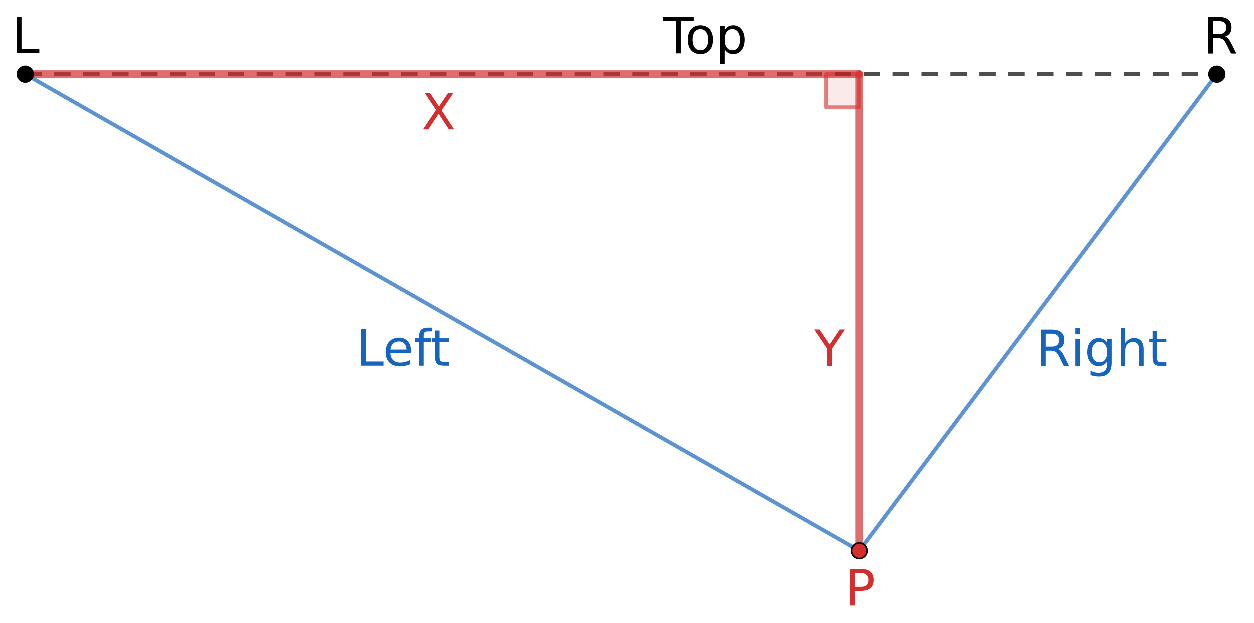
\includegraphics[width=.45\textwidth]{img/drowbot-maths.eps}
  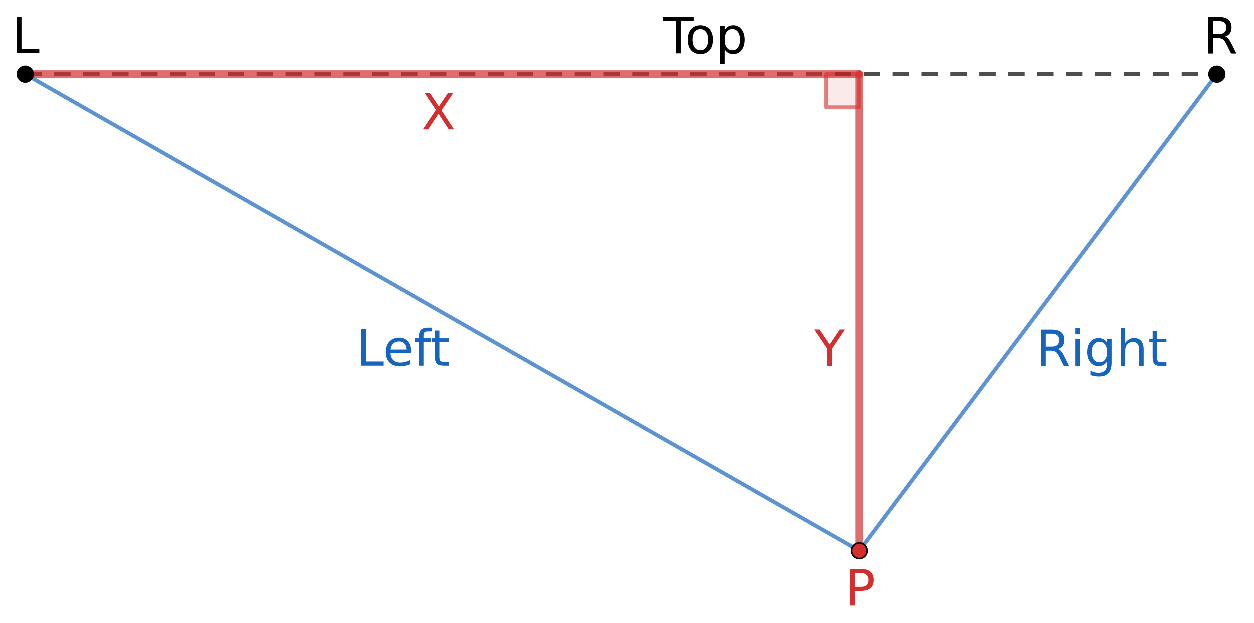
\includegraphics[width=.5\textwidth]{img/drowbot-maths.eps}
  \caption{Mapping polar to Cartesian coordinates.}
  \label{fig:maths}
% \end{wrapfigure}
\end{figure}

We colour coded the labels and lines in the example and will now
explain what they represent.
The black labels represent fixed constant values with $L$ and $R$
representing the stepper motors, and $Top$ the distance between them.
The blue $Left$ and $Right$ represent the chain lengths, which are
the only variables we control directly.
The red $P$ represents the platform at position $(X,Y)$ in Cartesian
coordinates.
One of the nice constraints in this case is that $P$ will never be
left of $L$ or right of $R$ and will always be below $L$ and $R$ due
to gravity. This helps simplify the calculations a bit.

Through calibration and manual measurement we know the lengths $Top$,
$Left$, and $Right$ and can use those to calculate the coordinates
for point $P$.
We shall start with $Y$, the height of the triangle $L,R,P$.

Getting the height of a triangle with known side lengths is simple.
We start with Heron's formula to calculate its area:
$$s = \frac{Top + Left + Right}{2}$$
$$Area = \sqrt{s(s-Top)(s-Left)(s-Right)}$$
%
Now we can solve the equation for the area of a triangle for the height:
$$Area = \frac{height \times base}{2} = \frac{Y \times Top}{2}$$
$$Y = \frac{2 \times Area}{Top}$$
%
We can then obtain the position of $X$ using the Pythagorean theorem:
$$X = \sqrt{Left^2 - Y^2}$$

Now that we know how to get from side length to coordinates we can
also go in the opposite direction and calculate how long $Left$ and
$Right$ need to be to get $P$ to a given $X,Y$.
This is another simple application of the Pythagorean theorem:
$$Left = \sqrt{X^2 + Y^2},\ Right = \sqrt{(Top - X)^2 + Y^2}$$

The interface we used for our demonstration was based on moving
in straight lines between two positions in the Cartesian coordinate
system, which is not as trivial as it might seem.
In the project overview we mentioned that polar plotters use a
bipolar coordinate system internally, which is a system that uses
the distances from two fixed centres to the target point as the
coordinates.

In our case that means that our internal position of $P$ is not
$(X,Y)$, but actually the integer values for $(Left,Right)$
which most closely approximate what would be the position $(X,Y)$
that the user provided.

% Micky: I'm not saying we should completely leave this part out, 
% but it may not be necessary to go into detail about our weaknesses.
% I know, I also have major problems leaving out information and feeling dishonest for it.
% However, you already pointed out the approximation in the paragraph above
% and I think we can leave it at that. Still too many pages...

%This disconnect means that moving from one Cartesian coordinate
%to another in a straight line does not translate in a smooth linear
%change for the bipolar system.
%Sadly we lacked the time to properly analyse and solve this in an
%elegant fashion so we went with the other approach to change the
%straight line into a series of small line segments in Cartesian
%coordinates and translating those to bipolar coordinates so the
%overall movement seems to be straight.
%Even though we did not use any microstepping for our prototype
%while our drivers did support it we already had a resolution of
%about half a millimetre per step and considering how relatively
%inaccurate chalk is the difference between this interpolation
%and an actual straight line is absolutely invisible.

\section{Conclusion and discussion}
\label{sec:conclusion}

% Micky: yep, modesty and self-deprecation can be saved for a much-needed later occasion :)

%In some miraculous fashion we managed to achieve all the lofty goals
%we set for this project.
%We have a functioning drawing robot that can read something from
%the blackboard and act based on whatever it saw on its own without
%direct input.

%This project was a lot of fun, but it also ended up costing both
%member a large part of the month we spent creating this.

% Micky: this one comes right out of my collection of standard NT sentences I keep in a yar.
The design of the Drowbot was challenging yet rewarding experience 
and we are glad to have met most of not all of the goals we had initially set.
Almost every step of the way we faced a new setback and almost all
of the initial parts of the design were replaced in the process.
The end result worked so much better than we could have dreamt,
especially considering all the setbacks.

Although we did end up with a working prototype, 
obviously still many improvements must be made in order arrive at a production model. 
Future work includes removing it from its blackboard and chalk
constraints and see what it can do on a medium that is
more controlled and easier to move in, such as ink on paper. 
Furthermore we believe that much more interesting algorithms can be devised 
where the optical feedback system could be even more useful.


\begin{thebibliography}{9}
%TODO: MORE CITING
% Micky: Added Wolfram/1d CA and Dragon curve

\bibitem{polargraphsite}
  \textit{Polargraph}, Sandy Noble
  \\\url{http://www.polargraph.co.uk/}

\bibitem{github}
  \textit{Drowbot GitHub repository}, Micky Faas, Koen Putman
  \\\url{https://github.com/mickymuis/drowbot}

\bibitem{elemca}
Wolfram, Stephen:
\textit{``Statistical mechanics of cellular automata."}
In: Reviews of Modern Physics, Vol. 55.3: 601--644.
(1983)

\bibitem{dragon}
\textit{Dragon Cuve} on Wolfram Mathworld
\\\url{http://mathworld.wolfram.com/DragonCurve.html}

\end{thebibliography}



\clearpage
\appendix

\section*{Photography}

\begin{figure}[h!]
  \centering
  \begin{subfigure}[t]{0.55\textwidth}
    \centering
    \includegraphics[height=15em]{img/ca_res.jpg}
    \caption{Result from drawing a cellular automaton with Wolfram code 22}
    \label{fig:ca_res}
  \end{subfigure}
  \begin{subfigure}[t]{0.4\textwidth}
    \centering
    \includegraphics[height=15em]{img/dragon_curve.jpg}
    \caption{A section of the dragon curve}
    \label{fig:drag_curve}
  \end{subfigure}
\end{figure}

\begin{figure}[h!]
  \centering
  \includegraphics{img/overview_rs.jpg}
  \caption{Drowbot deployed on a blackboard}
  \label{fig:overview}
\end{figure}

% Micky: Is this really necessary?
%\section{Physical Design}
%\label{sec:design}

% Appendix I: An overview of the system requirements.
\section{System requirements}
\label{sec:sysreq}
The general requirements are a lot of time on your hands and a wide
arrangement of tools, but we will go into more details about what
we used in this section.

% TODO: Is this comprehensive or did I forget some things
\subsection*{Motors and beaded chains}
\begin{itemize}
  \item A motor mount that can be clamped to the blackboard. We created brackets from wood and used five jigsaw clamps.
  \item NEMA 17 stepper motors (we used 1.8$^\circ$/step, 0.55N/M, 1.7A)
  \item Beaded chains (we used chrome, 4.4mm beads, 2mm apart)
  \item Several 3D printed parts (.stl available on GitHub)
  \begin{itemize}
    \item beaded chain pulleys for the stepper motors
    \item levers to attach the chains to bearings on the platform
    \item eyelets attach a counterweight to the chain
  \end{itemize}
  \item Counterweights (we used water bottles filled to aprox. 250 mL)
\end{itemize}

\subsection*{The gondola}
\begin{itemize}
  \item The platform itself (printable template SVG available)
  \item A Raspberry Pi Zero W or equivalent with
  \begin{itemize}
    \item at least 5 GPIO pins (2x step, 2x dir, 1x servo PWM)
    \item a picamera or other camera with V4L2 drivers
    \item an SD card with a Linux-based ARM OS (e.g. archlinuxarm)
    \item the ability to compile and use the PIGPIO library (or
          willingness to port the code to use some other GPIO library)
  \end{itemize}
  \item A custom shield for the Pi with
  \begin{itemize}
    \item A Female RJ45 connector to receive power and send signals
    \item Some way to connect the servo to power and the PWM pin
    \item Connections to several other GPIO pins for motor control
    \item Power distribution to the Pi and servo
    \item A 3.3V signal to send up from the Pi to the motor drivers
  \end{itemize}
  \item A servo to lift the chalk of the blackboard (like a MG996R). The template may need to be adapted for differently sized motors.
  \item A spring powered bar for the servo to push against. We used a bar made of 4 mm acrylate, with two M6 holes that line up with the corresponding holes in the gondola. Two springs and two long M6 hex bolts with ~30 mm flat shaft are also required.
  \item A camera mount for your camera. We used a PiCamera held by a piece of acrylate.
  \item A tube to mount the end-effector in (we used 10 mm chalk).
  \item Ball bearings to hold the chain handles. We used bearing that could fit over a 12 mm tube, measuring 32x10 on the outside. The OpenSCAD template can be easily modified to accommodate other sizes.
  \item M6 Nylon bolts to use as standoffs for the platform
  \item Standoffs to attach the Pi and the custom shield
  \item Many other nuts and bolts for various purposes, mainly to attach the camera (M3 for the platform, the PiCamera holes are M2).
  \item Some weight to hold the bottom of the platform down
\end{itemize}

\subsection*{Motor drivers and power delivery}
\begin{itemize}
  \item A power supply for the Pi/Servo (we used 5V USB with at least 2A)
  \item A motor power supply (we used one with 19V, 3.16A)
  \item A 100 \textmu F capacitor to smooth current between motor power and ground
  \item DRV8825 Stepper Motor Driver (or equivalent)
  \item Two RJ45 sockets to attach the Cat 5e cable
  \item We used protoboard to create a shield for the RasberryPi in order to route the used pins to the RJ45. The motors drivers are mounted on a second protoboard, also containing a female RJ45 socket and an micro-usb socket for 5V supply.
\end{itemize}

%Appendix II: Complete and very clear instructions on how to get your
% demo working.
\section{Build instructions}
\label{sec:buildinst}

\subsection{Building the gondola}

\begin{figure}[h!]
  \centering
  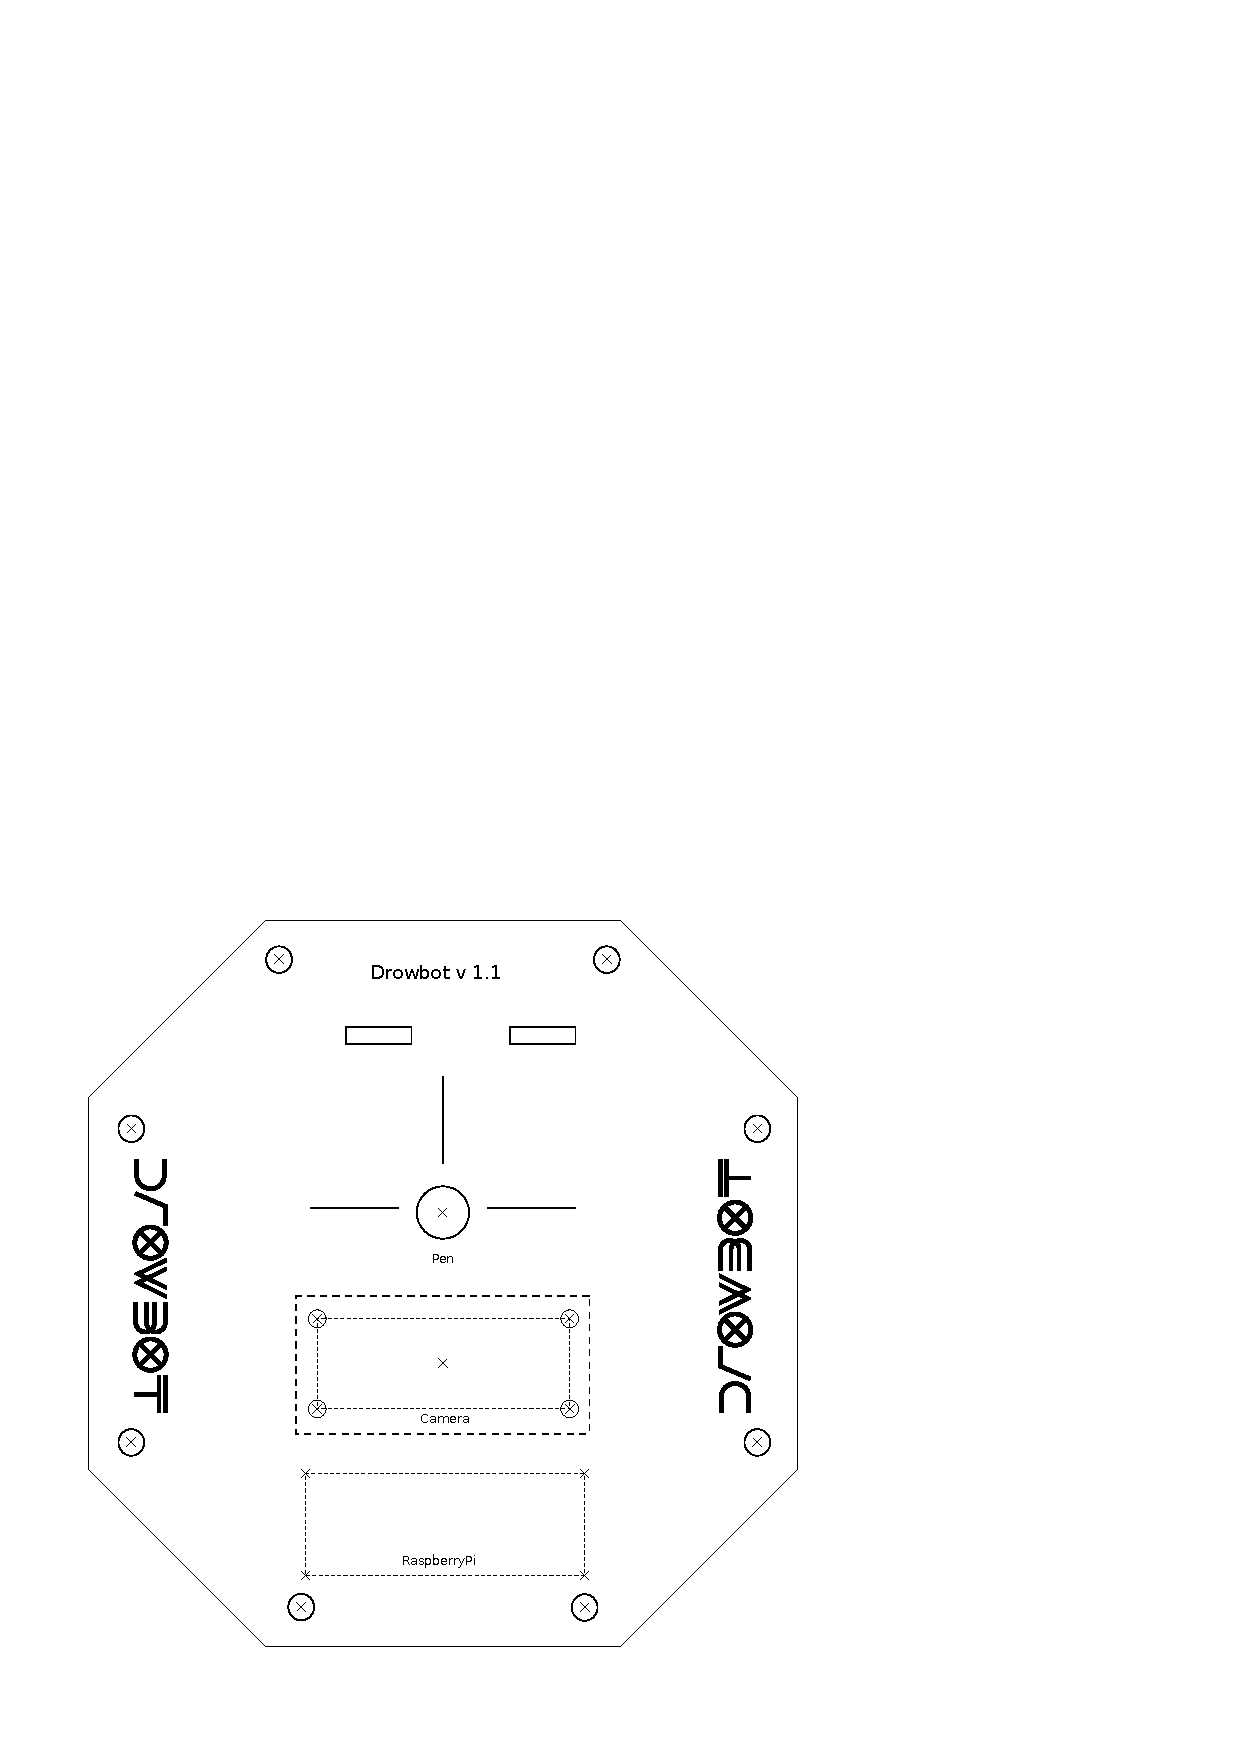
\includegraphics{img/gondola.jpg}
  \caption{Assembled and attached gondola}
  \label{fig:gondola}
\end{figure}


% Micky: ik heb maar PNG gedaan want ik had geen zin om met LaTeX te vechten om mijn SVGs...
\begin{figure}[h!]
  \centering
  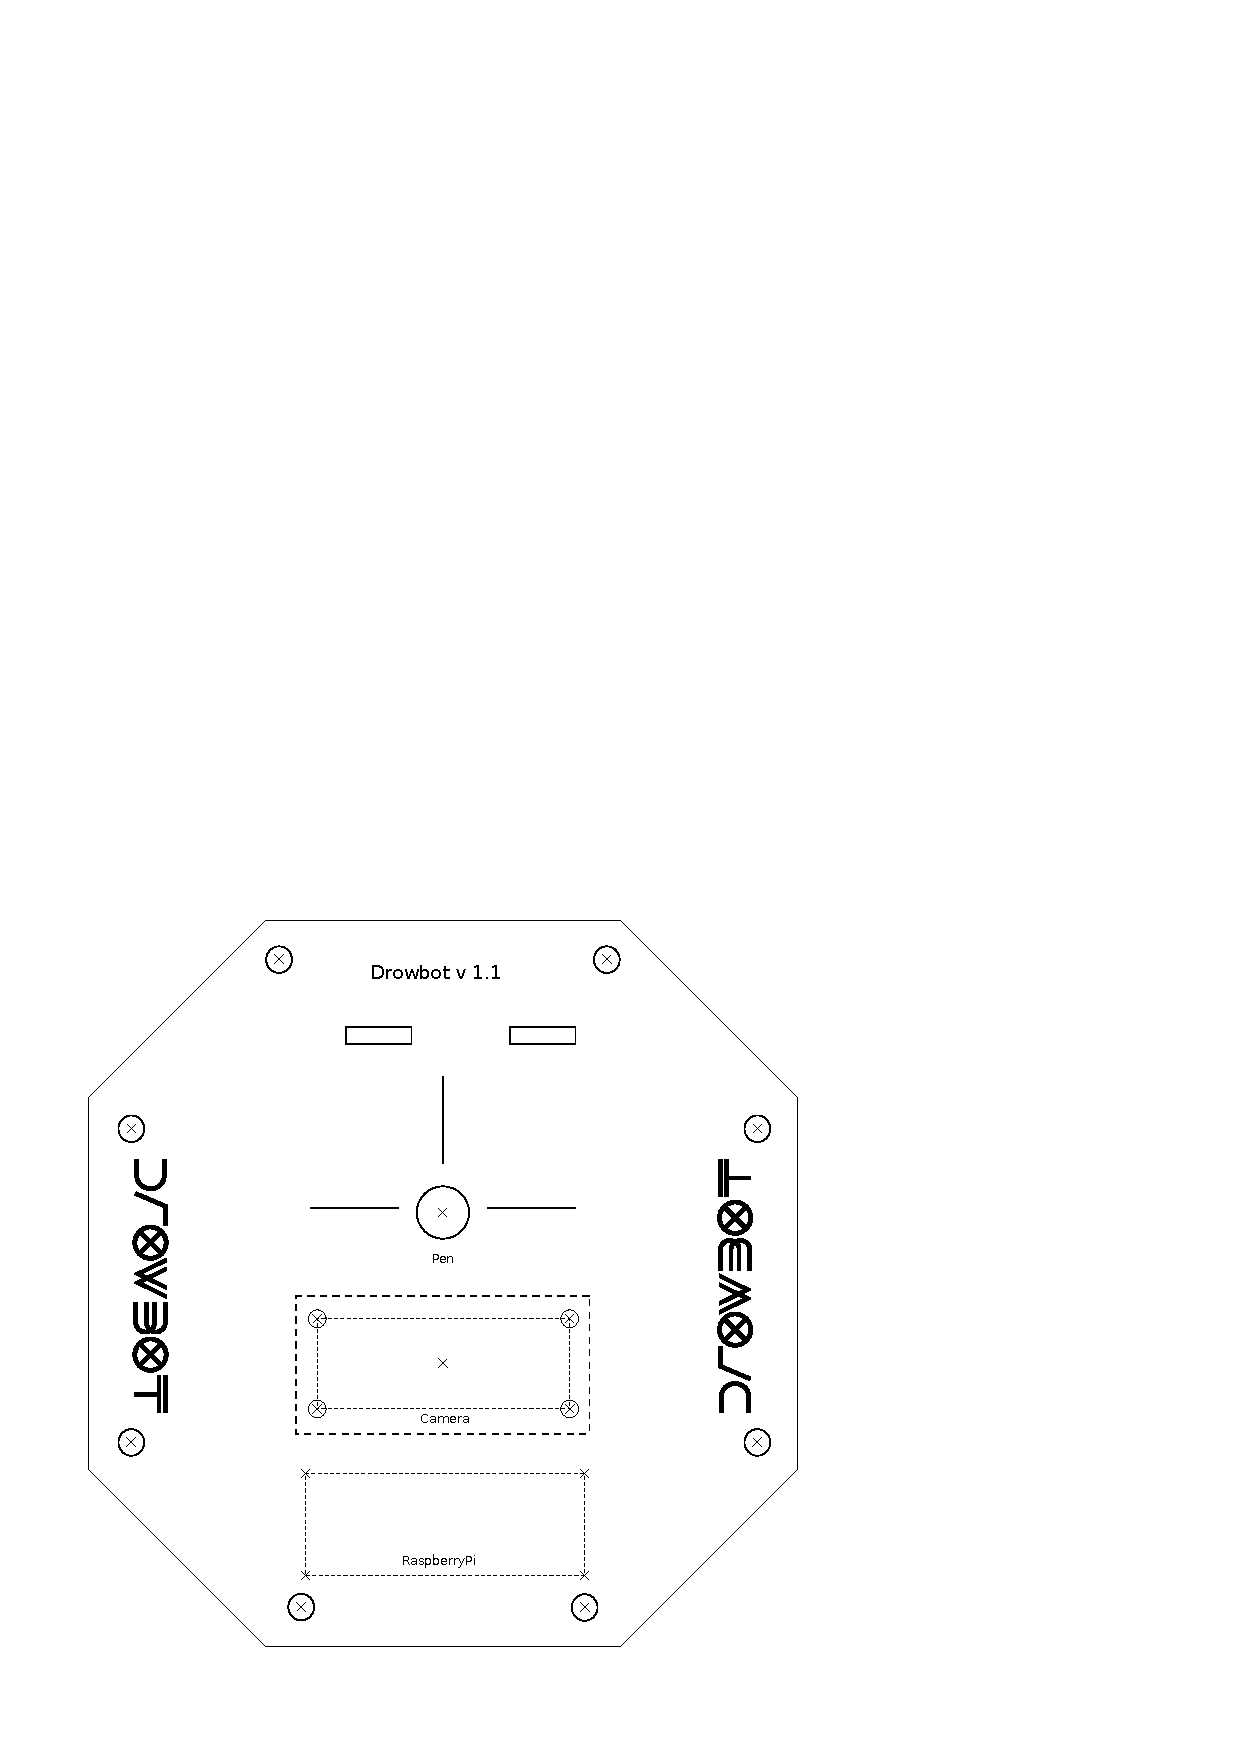
\includegraphics{img/gondola.png}
  \caption{Design template for the gondola baseplate}
  \label{fig:baseplate}
\end{figure}

\subsection{Building and attaching the motor suspensions}

\begin{figure}[h!]
  \centering
  \includegraphics{img/motorsusp.jpg}
  \caption{Assembled and attached motor suspensions}
  \label{fig:gondola}
\end{figure}

\subsection{Constructing and wiring the driver assembly}

\begin{figure}[h!]
  \centering
  \includegraphics{img/driverboard.jpg}
  \caption{Driver board with two DRV8825s, female RJ45, USB-power and separate motor power.}
  \label{fig:driverboard}
\end{figure}



\begin{figure}[h!]
  \centering
  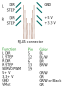
\includegraphics[scale=.75]{img/pinout.png}
  \caption{Pin-out used for the RJ45 wiring}
  \label{fig:pinout}
\end{figure}

% TODO: I forgot how detailed this had to be but it sure needs to happen
% TODO: ADD SPECS FOR EVERYTHING, or at least some wiring info

\end{document}

